% Template for Cogsci submission with R Markdown

% Stuff changed from original Markdown PLOS Template
\documentclass[10pt, letterpaper]{article}

\usepackage{cogsci}
\usepackage{pslatex}
\usepackage{float}
\usepackage{caption}

% amsmath package, useful for mathematical formulas
\usepackage{amsmath}

% amssymb package, useful for mathematical symbols
\usepackage{amssymb}

% hyperref package, useful for hyperlinks
\usepackage{hyperref}

% graphicx package, useful for including eps and pdf graphics
% include graphics with the command \includegraphics
\usepackage{graphicx}

% Sweave(-like)
\usepackage{fancyvrb}
\DefineVerbatimEnvironment{Sinput}{Verbatim}{fontshape=sl}
\DefineVerbatimEnvironment{Soutput}{Verbatim}{}
\DefineVerbatimEnvironment{Scode}{Verbatim}{fontshape=sl}
\newenvironment{Schunk}{}{}
\DefineVerbatimEnvironment{Code}{Verbatim}{}
\DefineVerbatimEnvironment{CodeInput}{Verbatim}{fontshape=sl}
\DefineVerbatimEnvironment{CodeOutput}{Verbatim}{}
\newenvironment{CodeChunk}{}{}

% cite package, to clean up citations in the main text. Do not remove.
\usepackage{apacite}

% KM added 1/4/18 to allow control of blind submission


\usepackage{color}

% Use doublespacing - comment out for single spacing
%\usepackage{setspace}
%\doublespacing


% % Text layout
% \topmargin 0.0cm
% \oddsidemargin 0.5cm
% \evensidemargin 0.5cm
% \textwidth 16cm
% \textheight 21cm

\title{Re-examining cross-cultural similarity judgements using lexical
co-occurrence}

\usepackage[utf8]{inputenc}
\usepackage[T1, T5]{fontenc}

\author{{\large \bf Morton Ann Gernsbacher (MAG@Macc.Wisc.Edu)} \\ Department of Psychology, 1202 W. Johnson Street \\ Madison, WI 53706 USA \AND {\large \bf Sharon J.~Derry (SDJ@Macc.Wisc.Edu)} \\ Department of Educational Psychology, 1025 W. Johnson Street \\ Madison, WI 53706 USA}

\newlength{\cslhangindent}
\setlength{\cslhangindent}{1.5em}
\newenvironment{CSLReferences}%
  {}%
  {\par}

\begin{document}

\maketitle

\begin{abstract}
Is ``cow'' more closely related to ``grass'' or ``chicken''? Speakers of
different languages judge similarity in this context differently, but
why? One possibility is that cultures co-varying with these languages
induce variation in conceptualizations of similarity. Specifically, East
Asian cultures may promote reasoning about thematic similarity, by which
cow and grass are more related whereas Western cultures may bias
similarity judgements toward taxonomic relations, like cow-chicken. This
difference in notions of similarity is the consensus interpretation for
cross-cultural variation in this paradigm. We consider, and provide
evidence for, an alternative possibility, by which notions of similarity
are equivalent across contexts, but the statistics of the environment
vary. On this account, similarity judgements are guided by co-occurrence
in experience, and observing or hearing about cows and grass or cows and
chickens more often could induce preferences for the relevant grouping,
and account for apparent differences in notions of similarity across
contexts.

\textbf{Keywords:}
similarity; culture; language; semantics; lexical co-occurrence;
variation
\end{abstract}

\hypertarget{introduction}{%
\section{Introduction}\label{introduction}}

By virtue of discrete words and grammatical features, language provides
a categorical partition of our continuous experiences. By measuring the
similarity between words (as commonly done with lexical co-occurrence
models), it may be possible to model the shape of similarity space in
order to capture cross-linguistic and cross-cultural variation and
provide a more general answer to the question of how language influences
our conception of the world.

Taxonomic and thematic similarity provide a convenient entry point to
broader debates about cross-linguistic and cross-cultural variation in
notions of similarity. Taxonomic categorization is based on the
similarity of attributes, for example, similar perceptual properties,
like shared color or shape, among objects. In contrast, thematic
categorization is based on causal, spatial, and temporal relationships
among objects (Markman \& Hutchinson, 1984). To illustrate this point,
if a participant is given the words ``chicken'' and ``grass'', and asked
which of those words are more closely related to the word ``cow'', the
pairing ``chicken'' - ``cow'' indicates a taxonomic match, whereas
``grass'' - ``cow'' indicates a thematic match.

Ji, Zhang, \& Nisbett (2004) found that preferences for taxonomic and
thematic matches differ across cultures, even when controlling for
testing language and fluency. Specifically, Chinese participants made
more thematic matches than taxonomic, while the converse was true for
European Americans. This difference held even for Chinese participants
tested in English (rather than Mandarin), suggesting that culture has an
effect on the categorization strategy independent of the test language.
However, the study also found an effect of language within Chinese
participants from mainland China (when tested both in China and in the
US): their preference for thematic categorization was significantly
lower when tested in English compared to Mandarin Chinese. This suggests
that test language also influences categorization strategies. Ji et
al.~characterize these results as demonstrating that culture
(independent of language) leads to different styles of reasoning about
similarity, whereas language serves as a ``tuning'' mechanism operating
within a culturally-specific style, by activating representations
corresponding to the language being used.

\hypertarget{cross-cultural-variation-in-similarity}{%
\subsection{Cross-cultural variation in
similarity}\label{cross-cultural-variation-in-similarity}}

The view that culture drives differences in categorization style has
been one favored by other non-linguistic studies that use taxonomic vs
thematic categorization to probe similarity judgment. When shown
pictorial triads that represent words (i.e.~pictures of an ant, a bee,
and honey), Chinese children (9-10 years old) scored higher on thematic
categorization compared to American children of the same age range, and
vice versa for taxonomic categorization (Chiu, 1972). These
cross-cultural differences in similarity judgment persist in novel
object categorization, with Chinese participants preferring to group by
family resemblance across multiple features and Americans preferring a
single-feature rule (Norenzayan, Smith, Kim, \& Nisbett, 2002). Since
differences in categorization style persist with novel stimuli (as
opposed to previously seen words or pictures of concepts), this suggests
that participants from different cultural backgrounds are utilizing
different reasoning strategies when making similarity judgments. The
authors attribute these differences to tendencies toward analytic
processing in Western cultures, which emphasizes objects and their
properties and holistic processing in East Asian cultures, which
emphasizes relationships between objects and their context. According to
this framework, East Asians attend more to relationships between objects
and context and reason more holistically, whereas Westerners attend more
to objects and their properties, and reason analytically (ibid, see also
Nisbett (2003)). In related work, East Asian participants show a higher
level of sensitivity to context than their Western counterparts when
reproducing drawings from memory (Ji, Peng, \& Nisbett, 2000); visually
exploring naturalistic scenes (Chua, Boland, \& Nisbett, 2005);
describing scenes (Masuda \& Nisbett, 2001); and in explaining the
causes of ambiguous behaviors (Choi, Nisbett, \& Norenzayan, 1999).
These cross-cultural differences in attention and analytic vs holistic
processing are seen to map onto the cross-cultural differences in
similarity judgment: because East Asian participants attend more to the
context between objects and reason more holistically, it stands to
reason that they would consider words that appear in the same context
(i.e.~thematically similar) to be more similar than
taxonomically-similar words.

This view ascribes cross-cultural differences in similarity judgment
tasks to variation in the conceptualization of similarity itself.
Alternatively, these judgments could be shaped by cross-cultural
differences in the statistics of the environment, and accordingly the
content of everyday experiences. Perhaps when confronted with the triad
task, participants from all cultures follow the same process for
reasoning about similarity, but rely on language or culture-specific
inputs to this process. For example, it may be that Vietnamese
participants are more likely to have knowledge of farming practices than
Americans, and may associate cows and grass more strongly (as grass is
the typical feed for cows in the small-scale family farming contexts
common in Vietnam). Americans, on the other hand, may have strong
associations between cows and chickens as a result of encountering them
together in children's books or petting zoo contexts. If we observe a
difference in categorization between, say Vietnamese and US
participants, it could be that members of both groups use the same
procedure (considering similarity that is influenced by both taxonomic
and thematic relations), but the inputs to this procedure differ between
cultures, with Vietnamese participants exposed to more instances of
``cow'' and ``grass'' occurring together, compared to US participants.

\hypertarget{language-as-a-proxy-of-variation-in-experience}{%
\subsection{Language as a proxy of variation in
experience}\label{language-as-a-proxy-of-variation-in-experience}}

While co-occurrences in experience are difficult to measure,
co-occurrence in language can provide a rough proxy--and indeed,
language may afford many of the ``experiences'' that people have with
infrequently encountered items, like cows or helicopters. In this study,
we use co-occurrence in language as a proxy of cultural experience. This
is a generalizing assumption, and while no linguistic corpus can be
expected to fully capture a culture, using this proxy as a model of
culture provides a conservative test of the hypothesis that differences
in the input, rather than the process, of reasoning produces cultural
variation in this task. This means that if such a model does work -- if
linguistic co-occurrence can predict cultural variation in this
similarity task without building differences in the decision process
into the model -- it is relatively strong evidence that language alone
(perhaps as a more easily observed source of information on broader
cultural and ecological variation) may account for these cross-cultural
differences in reasoning.\footnote{While we discuss cross-cultural
  variability at the level of countries or larger world areas, these are
  not cultural monoliths. For convenience, we operationalize culture at
  the level of country, based on where participants were raised. It is
  an open question whether performance in our participant populations
  (of relatively young and well-educated adults) is representative of
  the broader country. This is especially true for societies with
  substantial ethnic and cultural variation such as the US. We expect
  that our data is likely to underestimate variation both within and
  between the countries we sample from.}

Indeed, previous work suggests that using lexical co-occurrence as a
proxy can be useful in thinking about similarity judgments. Natural
language processing tasks have found that lexical co-occurrence is a
good predictor for performance in similarity judgment tasks. Griffiths,
Steyvers, \& Tenenbaum (2007) showed that a model that takes
word-document co-occurrence as input can be used to predict word
association and the effects of semantic association on a variety of
linguistic tasks. Additionally, lexical semantic models that are
constructed using lexical co-occurrence (as opposed to annotated
relations) have been shown to perform well on predicting human judgments
about similarity between word pairs that are either thematically or
taxonomically related (Rohde, Gonnerman, \& Plaut, 2006).

Our current study will be using 2 measures of lexical co-occurrence: 1)
raw lexical co-occurrences and 2) cosined distances of fastText word
vectors. fastText is a system that uses lexical co-occurrence
information to generate a vector representing each word in its lexicon
(Mikolov, Grave, Bojanowski, Puhrsch, \& Joulin, 2018). fastText uses a
continuous bag-of-words model, which takes into account a symmetric
window of words surrounding the word in question and maximizes the
log-likelihood of the probability of the word given its context.
Calculating the cosine-similarity between word vectors from fastText
gives us a score of how similar the contexts of these words are.
Therefore, words that occur in the same context (high lexical
co-occurrence) would have a larger cosine-similarity score.

It must be noted that fastText supplements the lexical co-occurrence
information by simultaneously training weight vectors for each position
relative to the word in question, as well as adding sub-word information
(bag-of-character n-gram vectors for each character forming the words).
The similarity judgment prediction given by fastText may be more higher
than a model using purely lexical co-occurrence information. However,
models that use only lexical co-occurrence information (with or without
a simple position weight system that gives more weight to words that are
closer to the word in question) also perform well in similarity
prediction tasks. For this study, due to the lack of large cleaned
corpora for Mandarin and Vietnamese, we are leveraging fastText
pre-trained models on the languages we are interested in Grave,
Bojanowski, Gupta, Joulin, \& Mikolov (2018).

Systems like fastText and word2vec have been demonstrated to be good
predictors for similarity judgments. Liu, Feng, Wu, Chan, \& Fulton
(2019) showed that fastText performed well as the data for a system
matching responses in a knowledge base by how similar they are to a
customer's query. A study by Jatnika, Bijaksana, \& Suryani (2019)
tested a word2vec model trained on the English wikipedia corpus against
353 word pairs labeled with similarity values based on human judgment.
The word2vec model correlates moderately with human judgment. fastText
has also been shown to be sensitive towards cultural effects on word
meanings: Thompson \& Lupyan (2020) applied fastText to
language-specific Wikipedia corpus (among others) to generate a
``semantic neighborhood'' of 1010 meanings in different languages. The
study showed that languages that are spoken by more similar cultures,
more geographically proximate and/or historically related had more
semantic neighborhoods that aligned. This is a proof of concept for our
use of fastText in different languages with varying levels of
relatedness.

\hypertarget{the-present-study}{%
\subsection{The present study}\label{the-present-study}}

Ji et al. (2004) suggest that the notion of similarity is what varies
across cultural groups, but it is quite possible that similarity is
regarded in the same way and it is actually the input to this similarity
judgment that varies across culture contexts. It might be possible to
gain traction on possible mechanisms by examining whether variation in
similarity judgments co-varies with environmental statistics that differ
across the cultural and linguistic contexts.

In this study, we ask whether variation in lexical co-occurrence can
account for the cross-context (culture and language) differences
observed in how people evaluate similarity. First, we attempt to
replicate Ji et al. (2004) by running a study comparing English speakers
in the US and Mandarin speakers in mainland China. Second, we evaluate
whether the differences observed between English and Mandarin speakers'
similarity judgments also extend to comparisons between English and
Vietnamese, by running a similar study between English speakers in the
US and Vietnamese speakers in Vietnam. Vietnam is a Southeast Asian
country that borders China and is historically greatly influenced by
Chinese culture (Hui, 2002). Therefore, it serves as a suitable cultural
context to investigate whether the claim made by Ji et al. (2004) and
previous studies, that Eastern and Western cultures have different
notions of similarity, extends beyond mainland China.

We then ask to what extent similarity judgments show cross-context
differences that align with co-occurrence patterns in participants'
languages. We would only see a main effect of cultural context if
differing notions of similarity drive these cross-cultural differences.
Meanwhile, if we do see variation in responding trial-to-trial that
tracks with lexical co-occurrence statistics (as a rough proxy combining
both linguistic and cultural context), this suggests that cross-cultural
notions of similarity might be similar, and it is environmental
statistics that guide the differences in similarity judgments. To
preview our results, we find that, while we do not see overall group
differences (between the East Asian contexts and the US) in similarity,
we do find language-specific co-occurrence can indeed explain
cross-context differences in similarity judgments. In contrast to
previous accounts, by which culture induces differing conceptions of
similarity (varying between taxonomic and thematic), these findings
provide an alternative, and more specific, account by which language may
explain these cross-cultural differences without invoking variation in
notions of similarity.

\hypertarget{methods}{%
\section{Methods}\label{methods}}

\hypertarget{participants}{%
\subsection{Participants}\label{participants}}

We recruited 200 participants from the US, 199 participants from
Vietnam, and 200 participants from mainland China. US participants were
recruited through snowball sampling seeded with Stanford student email
lists, Vietnam participants were recruited through snowball sampling
seeded with Vietnam-based student groups on Facebook, and mainland China
participants were recruited through snowball sampling seeded with group
chats on WeChat. US participants were compensated with \$5 gift
certificates (USD), VN participants received 50,000₫ (VND) in phone
credit, and mainland China participants received 25CNY through WeChat
credit transfer.

We excluded 8 US participants, 62 Vietnam participants, and 34 China
participants who did not answer all attention checks correctly. We
followed 4 exclusion criteria that aim to retain only participants who
are influenced by one culture: (1) non-native speakers of English and
Vietnamese, respectively, (2) fluent in at least one of the other two
study languages (Vietnamese for US participants, English for Vietnamese
participants and Chinese participants), (3) have lived outside of the
test country (US, Vietnam, or China) for more than two years, and (4)
have significant international experience (more than 6 international
experiences of 2 days or longer.) We did not use a particular criterion
for a language if it would exclude 25\% or more of any one sample. In
this round of exclusion, we excluded 68 US, 27 Vietnam participants, and
34 China participants. After these exclusions, the US sample included
124 participants (30M, 89F, 3 non-binary, 2 other), with mean age =
22.18 (SD = 8) and median age = 20. The Vietnam sample included 110
participants (34M, 71F, 5 other), with mean age = 22.21 (SD = 5.81) and
median age = 21. The China sample included 132 participants (51M, 81F,
other), with mean age = 23.27 (SD = 3.75) and median age = 23.

Notably, we lost a majority of our Vietnam participants (more than 60\%)
in the attention check exclusion. One reason we suspect why this might
have happened is because our Vietnam participants are less familiar with
research surveys and attention check questions, and thus might have
thought too much about the attention check questions. We carried out an
exploratory analysis where we used a less stringent attention check
exclusion (covered in the final part of the Results \& Analysis
section). To preview our findings for this analysis, we did not find any
difference in significant results when compared with the main analysis.

\hypertarget{stimuli}{%
\subsection{Stimuli}\label{stimuli}}

We adapted stimuli from previous studies to create a set of test triads
consisting of a cue, with one thematic and one taxonomic match option.
For example, ``cow,'' ``grass,'' and ``chicken,'' where ``cow'' is the
cue, ``grass'' is the thematic match, and ``chicken'' the taxonomic
match. We included 105 such triads, a superset including triads pulled
from supplemental information and in-text examples across the
literature, and others that we adapted or created (see SI for the full
list of stimuli and sources). We selected triads on the basis of
cultural familiarity in the US, Vietnam, and China. The triads were
originally in English; they were translated to Vietnamese and Mandarin
by a fluent bilingual speaker in each language. The translations were
then checked for accuracy after backtranslation to English by another
fluent bilingual in each language who was naive to the original English
versions.

Each participant completed all 105 triads in sets of 21 trials at a time
(10 test triads, 10 filler triads, and 1 attention check per page), by
selecting the match most related to the cue (``Which thing is most
closely related to the bolded item?'' or ``Thứ nào liên quan nhất với
thứ được in đậm?''). The test triads were presented with 105 filler
triads mixed in, to obscure the taxonomic-thematic two-answer forced
choice structure of the test stimuli and reduce the likelihood that
participants would become aware of the design. The filler triads were
groups of three semantically related words, but where the match options
were not distinguished by thematic vs.~taxonomic similarity, e.g., cue
``bird'' with match options ``lizard'' and ``toad.'' Additionally, we
included 10 attention check trials, which were formatted like the test
and filler triads but included an instruction instead of a cue item,
e.g., ``Choose wife'' with match options ``wife'' and ``husband.'' In
total, each participant completed 210 similarity judgments and 10
attention check questions, with triads presented in randomized orders
that varied between subjects.

\hypertarget{corpus-model}{%
\subsection{Corpus model}\label{corpus-model}}

Our general approach is to build a model of similarity that is based on
collocation counts in each language.

\hypertarget{raw-lexical-co-occurrences}{%
\subsubsection{Raw lexical
co-occurrences}\label{raw-lexical-co-occurrences}}

To give an intuition for our model, consider the cow-grass-chicken
triad: we counted how many times ``cow'' and ``grass'' co-occur within a
window of text in each corpus, and compare this to how many times
``cow'' and ``chicken'' co-occur. Our similarity prediction is then
proportional to the relative frequency of these pairs. For example, if
the thematic cow-grass match accounts for 30\% of collocations for this
triad (with cow-chicken making up the other 70\%), then our model
predicts, correspondingly, that 30\% of responses to the triad will be
grass, and the other 70\% chicken. We then use a mixed-effects
regression to evaluate how well each corpus collocate model predicts
participants' similarity judgments, across triads and languages.

\hypertarget{collocate-retrieval-and-coding}{%
\paragraph{Collocate retrieval and
coding}\label{collocate-retrieval-and-coding}}

For our English co-occurrence metric, we used the online interface of
the Corpus of Contemporary American English (Davies, 2008-) to retrieve
collocation counts. We recorded the raw count of times that any
cue-match pair (e.g., cow-grass or cow-chicken) co-occur in a window of
19 words, which is the maximum window size in the online interface, and
closest to the sentence co-occurrence metric in our VI corpus
collocation counts.

To determine Vietnamese co-occurrence, we used the raw frequency of
sentence co-occurrences from a subset of the Vietnamese corpus in the
Leipzig Corpora Collection (Goldhahn, Eckart, \& Quasthoff, 2012); this
corpus includes 70 million Vietnamese sentences, but our corpus data
comes from a 1 million sentence subset for which co-occurrence counts
are available for download. Vietnamese makes very frequent use of
compositional morphology but the written language uses spacing to
delineate syllable boundaries rather than word boundaries. Accordingly,
collocate searches returned instances of both target terms and many
morphologically related, but distinct, words. We included in our counts
any instances of the target term or close semantic neighbors containing
the same morpheme(s) as long as they entailed a likely literal reference
to the target term. For example, our search for collocates of the term
``gà'' (chicken) also returned ``gà mái,'' a distinct word for female
chickens. Despite being a different word, ``gà mái'' both includes the
morpheme for ``chicken'' and entails reference to a chicken.
Accordingly, instances of both ``gà'' and ``gà mái'' were included in
our collocate count for ``chicken.'' Some compounds do not meet this
criteria, and were excluded from collocate counts. For example ``trái
cây'' (tree.fruits) includes the same syllable as the word ``cây''
(tree), but refers to fruit that comes from trees, not the trees
themselves, and was therefore excluded from our collocate counts for
``tree.''

TODO; ADD INFO ABOUT MANDARIN CORPUS

\hypertarget{collocate-similarity-model}{%
\paragraph{Collocate similarity
model}\label{collocate-similarity-model}}

From the raw co-occurrence counts of each triad, we calculated the
thematic co-occurrence ratio as the number of thematic co-occurrences
over the sum of thematic and taxonomic co-occurrences. We did this for
both the English and Vietnamese corpus co-occurrence counts. In this
way, we obtained predictions for 73 of 105 triads from the Vietnamese
corpus and 104 of 105 triads from English. We therefore limited all
analyses reported here to the subset of triads for which our
corpus-based model can make meaningful predictions, meaning triads that
have at least one non-zero collocate count (either thematic or taxonomic
match). We replaced any remaining zero collocate counts with
\(\epsilon\) to account for sparsity in the corpus data. We then tested
whether these simple relative frequency models predict US and VN
responding.

\hypertarget{cosine-distance-of-word-vectors}{%
\subsubsection{Cosine distance of word
vectors}\label{cosine-distance-of-word-vectors}}

To give an intuition for our model, consider again the cow-grass-chicken
triad: we retrieved word vectors for ``cow'' and ``grass'', and
calculate the cosine distance between these vectors. Similarly, we
retrieved vectors for ``cow'' and ``chicken'' and calculate the cosine
distance between them. Our similarity prediction is then inversely
proportional to the cosine distance of these pairs. This is because a
larger cosine distance means the word vectors are further apart, and
thus the words are less similar. For example, if the cosine distance of
thematic cow-grass is 0.7 and the cosine distance of taxonomic
cow-chicken is 0.3, then our model predicts, correspondingly, that 30\%
of responses to the triad will be grass, and the other 70\% chicken. We
then use a mixed-effects regression to evaluate how well each corpus
model predicts participants' similarity judgments, across triads and
languages.

\hypertarget{collocate-retrieval}{%
\paragraph{Collocate retrieval}\label{collocate-retrieval}}

We use the fastText pre-trained models of English, Mandarin, and
Vietnamese in Grave et al. (2018). These models are trained on Common
Crawl and Wikipedia using We distribute pre-trained word vectors for 157
languages, trained on Common Crawl and Wikipedia using fastText. These
models were trained using a Continuous Bag of Words (CBOW) with
position-weights and a window of size 5. The models use character
n-grams of length 5 and 10 negative examples.From the aforementioned
models, we retrieve the word vectors (dimension 300) for each word we
are interested in.

\hypertarget{collocate-similarity-model-1}{%
\paragraph{Collocate similarity
model}\label{collocate-similarity-model-1}}

From the word vectors, we calculated the cosine distance between each
cue-thematic match (thematic cosine distance) and cue-taxonomic match
(taxonomic cosine distance), using the spatial.distance.cosine function
from the SciPy package (Virtanen et al., 2020). We then calculated the
thematic cosine distance proportion as thematic cosine distance over the
sum of taxonomic cosine distance and thematic cosine distance. We did
this for all three corpora. We were able to obtain predictions for all
triads in all languages.

\hypertarget{results}{%
\section{Results}\label{results}}

\hypertarget{do-we-extend-previous-work-reporting-a-preference-for-taxonomic-matching-in-the-us-and-thematic-matching-in-asia}{%
\subsection{1. Do we extend previous work reporting a preference for
taxonomic matching in the US and thematic matching in
Asia?}\label{do-we-extend-previous-work-reporting-a-preference-for-taxonomic-matching-in-the-us-and-thematic-matching-in-asia}}

The group means of proportion of thematic response in mainland China is
the highest (M = 0.65, SD = 0.12), followed by the groups means in
Vietnam (M = 0.6, SD = 0.11), which is slightly higher than that of the
US (M = 0.57, SD = 0.16).

\begin{CodeChunk}
\begin{figure}[tb]
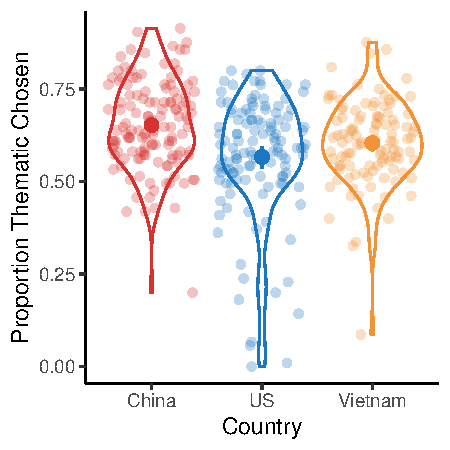
\includegraphics{figs/unnamed-chunk-2-1} \caption[Proportion of thematic responses by country]{Proportion of thematic responses by country. Only US-China responding comparison shows a siginficant difference. We could not extend this to US-Vietnam responding comparison.}\label{fig:unnamed-chunk-2}
\end{figure}
\end{CodeChunk}

To test for cross-context differences in similarity judgments between
the countries, we ran a mixed-effects logistic regression predicting
triad responding (taxonomic or thematic) with country (US, China, or
Vietnam) as a fixed effect. As random effects, we included an intercept
per subject and one per triad, as well as by-triad random slopes for
country to account for variation in the country effect across triads. In
R syntax, the model is: response \textasciitilde{} country + (1
\textbar{} subject) + (country \textbar{} triad).

Overall, there is a significant effect of country on proportion of
thematic responses (\(\chi^2\)(2) = 15.75, p \textless{} .001). However,
this effect is driven by the difference between US and China responding
(\(\beta\) = -0.5, p \textless{} .001). There is no statistical
difference between the Vietnam and China responding (\(\beta\) = -0.25,
p = 0.066), and the US and Vietnam responding (\(\beta\) = 0.25, p =
0.095).

On this analysis, we do not find support that the US-China tendencies
toward taxonomic and thematic responding (respectively) extend to the
US-Vietnam comparison. Accordingly, we cannot speak to overall biases
toward thematic responding across Asian cultural contexts broadly, but
we do replicate the differences documented by Ji et al. (2004) between
the US and China. However, in our corpus model comparison, we do find
evidence for different, more fine-grained variation in similarity
judgments between the US and Vietnam.

\hypertarget{can-the-differences-in-similarity-judgments-between-english-mandarin-and-vietnamese-speakers-be-explained-by-variation-in-lexical-statistics}{%
\subsection{2. Can the differences in similarity judgments between
English, Mandarin and Vietnamese speakers be explained by variation in
lexical
statistics?}\label{can-the-differences-in-similarity-judgments-between-english-mandarin-and-vietnamese-speakers-be-explained-by-variation-in-lexical-statistics}}

\hypertarget{is-responding-in-each-cultural-context-predicted-by-the-corresponding-lexical-statistics-raw-co-occurrences}{%
\subsubsection{Is responding in each cultural context predicted by the
corresponding lexical statistics (raw
co-occurrences)?}\label{is-responding-in-each-cultural-context-predicted-by-the-corresponding-lexical-statistics-raw-co-occurrences}}

\hypertarget{raw-lexical-co-occurrences-1}{%
\paragraph{Raw lexical
co-occurrences}\label{raw-lexical-co-occurrences-1}}

To test whether variation in lexical co-occurrence can explain
differences in similarity judgments between US and Vietnam participants,
we compare logistic mixed-effects regression models fit to the thematic
responding data from each country separately. We first ask how well each
corpus model (English, Vietnamese, or Mandarin) predicts similarity
judgments by speakers of the corresponding language (US, Vietnam, or
China). To do this, we use a mixed-effects logistic regression to
predict triad responses (0=taxonomic or 1=thematic) with corpus
prediction (proportion thematic co-occurrence or cosine distance) as a
fixed effect and participant and triad as random effects.

We found that all corpora are significant predictors of all cultural
context responding.

For US responding: English (EN), Vietnamese (VI), and Mandarin (ZH)
corpus are all significant predictors. EN corpus: \(\beta\) = 2.01,
\(\chi^2\)(1) = 17.42, p \textless{} .001. VI corpus: \(\beta\) = 1.21,
\(\chi^2\)(1) = 11.1, p \textless{} .001. ZH corpus: \(\beta\) = 1.15,
\(\chi^2\)(1) = 6.38, p = 0.012.

For Vietnam responding: English (EN), Vietnamese (VI), and Mandarin (ZH)
corpus are all significant predictors. EN corpus: \(\beta\) = 1.73,
\(\chi^2\)(1) = 12.35, p \textless{} .001. VI corpus: \(\beta\) = 1.27,
\(\chi^2\)(1) = 12.83, p \textless{} .001. ZH corpus: \(\beta\) = 1.8,
\(\chi^2\)(1) = 18, p \textless{} .001.

For China responding: English (EN), Vietnamese (VI), and Mandarin (ZH)
corpus are all significant predictors. EN corpus: \(\beta\) = 1.21,
\(\chi^2\)(1) = 9.83, p = 0.002. VI corpus: \(\beta\) = 0.77,
\(\chi^2\)(1) = 7.44, p = 0.006. ZH corpus: \(\beta\) = 1.15,
\(\chi^2\)(1) = 13.28, p \textless{} .001.

This suggests a strong shared similarity signal across the languages.

\hypertarget{cosine-distances-of-fasttext-word-vectors}{%
\paragraph{Cosine distances of fastText word
vectors}\label{cosine-distances-of-fasttext-word-vectors}}

Similar to the results from the analysis with raw lexical
co-occurrences, we found that all corpora are significant predictors of
all cultural context responding.

For US responding: English (EN), Vietnamese (VI), and Mandarin (ZH)
corpus are significant predictors of US responding (EN-US model:
\(\beta\) = -8.64, \(\chi^2\)(1) = 30.44, p \textless{} .001; VI-US
model: \(\beta\) = -2.97, \(\chi^2\)(1) = 5.23, p = = 0.022; ZH-US
model: \(\beta\) = -6.96, \(\chi^2\)(1) = 18.08, p \textless{} .001).

For Vietnam (VN) responding: English (EN), Vietnamese (VI), and Mandarin
(ZH) corpus are significant predictors of VN responding (EN-VN model:
\(\beta\) = -5.33, \(\chi^2\)(1) = 9.39, p = 0.002; VI-VN model:
\(\beta\) = -3.46, \(\chi^2\)(1) = 6.64, p = = 0.01; ZH-VN model:
\(\beta\) = -6.37, \(\chi^2\)(1) = 13.93, p \textless{} .001).

For China (CN) responding: English (EN), Vietnamese (VI), and Mandarin
(ZH) corpus are significant predictors of CN responding (EN-CN model:
\(\beta\) = -6.18, \(\chi^2\)(1) = 25.34, p \textless{} .001; VI-CN
model: \(\beta\) = -2.44, \(\chi^2\)(1) = 5.83, p = = 0.016; ZH-CN
model: \(\beta\) = -7.36, \(\chi^2\)(1) = 37.45, p \textless{} .001).

\hypertarget{is-responding-in-each-cultural-context-best-predicted-by-the-corresponding-corpuss-lexical-statistics-raw-co-occurrences-as-opposed-to-the-other-two-corpora}{%
\subsubsection{\texorpdfstring{Is responding in each cultural context
\textbf{best} predicted by the corresponding corpus's lexical statistics
(raw co-occurrences), as opposed to the other two
corpora?}{Is responding in each cultural context best predicted by the corresponding corpus's lexical statistics (raw co-occurrences), as opposed to the other two corpora?}}\label{is-responding-in-each-cultural-context-best-predicted-by-the-corresponding-corpuss-lexical-statistics-raw-co-occurrences-as-opposed-to-the-other-two-corpora}}

Next, we directly compare the corpus models by including both as fixed
effects in three mixed-effect regressions (predicting US, Vietnam and
China responding) with the same random effects as above. In R syntax,
the model is: response \textasciitilde{} corpus\_English +
corpus\_Vietnamese + corpus\_Mandarin + (1\textbar triad) +
(1\textbar subject).

\hypertarget{raw-co-occurrences}{%
\paragraph{Raw co-occurrences}\label{raw-co-occurrences}}

When we included all corpora thematic cosine distance proportion as
predictors, all corpora are significant in predicting all cultural
context's responding.

For US responding: only English (EN) corpus is a significant predictor.
EN corpus: \(\beta\) = 1.62, \(\chi^2\)(1) = 4.59, p = 0.032. VI corpus:
\(\beta\) = 0.46, \(\chi^2\)(1) = 1.04, p = 0.307. ZH corpus: \(\beta\)
= -0.03, \(\chi^2\)(1) = 0, p = 0.962.

For Vietnam responding: only English (EN) and Mandarin (ZH) corpora are
significant predictors. EN corpus: \(\beta\) = -0.02, \(\chi^2\)(1) = 0,
p = 0.979. ZH corpus: \(\beta\) = 1.39, \(\chi^2\)(1) = 6.5, p =
0.011.VI corpus: \(\beta\) = 0.79, \(\chi^2\)(1) = 3.3, p = 0.069.

For China responding: only Mandarin (ZH) corpus is a significant
predictor. ZH corpus: \(\beta\) = 0.9, \(\chi^2\)(1) = 4.31, p = 0.038.
EN corpus: \(\beta\) = 0.21, \(\chi^2\)(1) = 0.13, p = 0.72. VI corpus:
\(\beta\) = 0.35, \(\chi^2\)(1) = 1.02, p = 0.312.

\begin{CodeChunk}
\begin{figure}[tb]
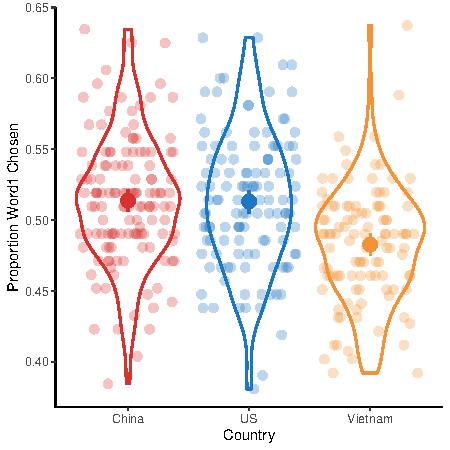
\includegraphics{figs/unnamed-chunk-4-1} \caption[Fixed effect sizes of each corpus when included as a predictor for China, US, and Vietnam responding, respectively]{Fixed effect sizes of each corpus when included as a predictor for China, US, and Vietnam responding, respectively. The English corpus is the best predictor for US response, and the Mandarin corpus is the best predictor for China response.}\label{fig:unnamed-chunk-4}
\end{figure}
\end{CodeChunk}

We observed some level of language specificity from this analysis. The
English corpus is the best predictor for US responding, and the Mandarin
corpus is the best predictor for China response. While this is not the
case with the Vietnamese corpus and the Vietnam responding, the
Vietnamese corpus is still a significant predictor for the Vietnam
responding.

However, we found that language specificity alone does not explain our
results. We used an ANOVA to compare the model with only the
corresponding corpus, and the model with all 3 corpora for each cultural
context. We found that in all three cases (US, China, Vietnam), adding
the other two corpora produces a significantly better fit than the
identical model without the additional corpora, and only the
corresponding corpus included as a predictor (US response: \(\chi^2\)(2)
= 1.04, p = 0.595; Vietnam response: \(\chi^2\)(2) = 8.84, p = 0.012;
China response: \(\chi^2\)(2) = 2.13, p = 0.345).

\_TODO: should we take this out?\_\_ We carried out an ANOVA model
comparison to compare our approach with previous studies that did not
include corpus information. Because Ji et al. (2004) only compared US
and China participants, we filtered our data to only include responding
data from these two countries. Our approach would be to compare a model
that only includes country (US or China) as a fixed effect with one that
also includes English and Chinese corpus data. Our previous model with
an intercept per subject and one per triad, as well as by-triad random
slopes for country to account for variation in the country effect across
triads fails to converge with the more complex model, so we include a
simpler random effect structure with an intercept per subject and one
per triad in both the basic and more complex model. We compare this
model with an identical model but including Chinese and English corpus
cosine distance proportion prediction. We found that adding English and
Chinese corpus data produces a significantly better fit than the
identical model without English and Chinese corpus data as predictors
(\(\chi^2\)(2) = 42.57, p = \textless{} .001. This suggests that
including corpus data would better model the cross-cultural differences
in similarity judgment in this study as well as similar studies.

\hypertarget{cosine-distances-of-fasttext-word-vectors-1}{%
\paragraph{Cosine distances of fastText word
vectors}\label{cosine-distances-of-fasttext-word-vectors-1}}

When we included all corpora thematic cosine distance proportion as
predictors, all corpora are significant in predicting all cultural
context's responding.

For US responding: English (EN), Vietnamese (VI), and Mandarin (ZH)
corpus are all significant predictors. EN corpus: \(\beta\) = -6.9,
\(\chi^2\)(1) = 17.06, p \textless{} .001. VI corpus: \(\beta\) = -2.18,
\(\chi^2\)(1) = 3.72, p = = 0.054. ZH corpus: \(\beta\) = -3.2,
\(\chi^2\)(1) = 3.59, p = = 0.058.

For Vietnam responding: English (EN), Vietnamese (VI), and Mandarin (ZH)
corpus are all significant predictors. EN corpus: \(\beta\) = -2.98,
\(\chi^2\)(1) = 2.58, p = = 0.108. VI corpus: \(\beta\) = -2.75,
\(\chi^2\)(1) = 4.84, p = = 0.028. ZH corpus: \(\beta\) = -4.39,
\(\chi^2\)(1) = 5.43, p = = 0.02.

For China responding: English (EN), Vietnamese (VI), and Mandarin (ZH)
corpus are all significant predictors. EN corpus: \(\beta\) = -3.52,
\(\chi^2\)(1) = 7.81, p = = 0.005. VI corpus: \(\beta\) = -1.62,
\(\chi^2\)(1) = 3.59, p = = 0.058. ZH corpus: \(\beta\) = -5.35,
\(\chi^2\)(1) = 17.28, p = \textless{} .001.

We observed some level of language specificity from this analysis. The
English corpus is the best predictor for US responding, and the Mandarin
corpus is the best predictor for China response. While this is not the
case with the Vietnamese corpus and the Vietnam responding, the
Vietnamese corpus is still a significant predictor for the Vietnam
responding.

\begin{CodeChunk}
\begin{figure}[tb]
\includegraphics{figs/unnamed-chunk-5-1} \caption[Fixed effect sizes of each corpus when included as a predictor for China, US, and Vietnam responding, respectively]{Fixed effect sizes of each corpus when included as a predictor for China, US, and Vietnam responding, respectively. The English corpus is the best predictor for US response, and the Mandarin corpus is the best predictor for China response.}\label{fig:unnamed-chunk-5}
\end{figure}
\end{CodeChunk}

However, we found that language specificity alone does not explain our
results. We used an ANOVA to compare the model with only the
corresponding corpus, and the model with all 3 corpora for each cultural
context. We found that in all three cases (US, China, Vietnam), adding
the other two corpora produces a significantly better fit than the
identical model without the additional corpora, and only the
corresponding corpus included as a predictor (US response: \(\chi^2\)(2)
= 7.95, p = = 0.019; Vietnam response: \(\chi^2\)(2) = 13.72, p = =
0.001; China response: \(\chi^2\)(2) = 10.83, p = NA).

\_TODO: should we take this out?\_\_ We carried out an ANOVA model
comparison to compare our approach with previous studies that did not
include corpus information. Because Ji et al. (2004) only compared US
and China participants, we filtered our data to only include responding
data from these two countries. Our approach would be to compare a model
that only includes country (US or China) as a fixed effect with one that
also includes English and Chinese corpus data. Our previous model with
an intercept per subject and one per triad, as well as by-triad random
slopes for country to account for variation in the country effect across
triads fails to converge with the more complex model, so we include a
simpler random effect structure with an intercept per subject and one
per triad in both the basic and more complex model. We compare this
model with an identical model but including Chinese and English corpus
cosine distance proportion prediction. We found that adding English and
Chinese corpus data produces a significantly better fit than the
identical model without English and Chinese corpus data as predictors
(\(\chi^2\)(2) = 42.57, p = \textless{} .001. This suggests that
including corpus data would better model the cross-cultural differences
in similarity judgment in this study as well as similar studies.

\hypertarget{does-similarity-reasoning-differ-across-cultures-only-the-input-to-it-or-both}{%
\subsection{3. Does similarity reasoning differ across cultures, only
the input to it, or
both?}\label{does-similarity-reasoning-differ-across-cultures-only-the-input-to-it-or-both}}

Does adding country and interaction term with the corresponding corpus
improves the model?

Adding country improves the model. Only country and interaction between
country and corresponding corpus's lexical co-occurrence are significant
predictors. Corresponding corpus's lexical co-occurrence is no longer a
significant predictor.

\hypertarget{how-general-are-the-cross-language-differences-in-similarity-judgments-we-observe-are-they-limited-to-taxonomic-thematic-contrasts-or-do-they-extend-to-other-cases}{%
\subsection{5. How general are the cross-language differences in
similarity judgments we observe? Are they limited to taxonomic-thematic
contrasts or do they extend to other
cases?}\label{how-general-are-the-cross-language-differences-in-similarity-judgments-we-observe-are-they-limited-to-taxonomic-thematic-contrasts-or-do-they-extend-to-other-cases}}

\begin{CodeChunk}
\begin{figure}[tb]
\includegraphics{figs/unnamed-chunk-8-1} \caption[Proportion of thematic responses by country]{Proportion of thematic responses by country. Only US-China responding comparison shows a siginficant difference. We could not extend this to US-Vietnam responding comparison.}\label{fig:unnamed-chunk-8}
\end{figure}
\end{CodeChunk}

No effect of country on filler responding.

\hypertarget{does-lexical-statistics-for-fillers-predict-responding-in-the-corresponding-cultural-context}{%
\subsubsection{Does lexical statistics for fillers predict responding in
the corresponding cultural
context?}\label{does-lexical-statistics-for-fillers-predict-responding-in-the-corresponding-cultural-context}}

\hypertarget{raw-co-occurrences-1}{%
\paragraph{Raw co-occurrences}\label{raw-co-occurrences-1}}

Yes, corpus raw co-occurrences predicts responding for both US and
Vietnamese. \emph{need to discuss with Shan to incorporate Mandarin due
to a lot of empty counts}

\hypertarget{cosine-distance}{%
\paragraph{Cosine distance}\label{cosine-distance}}

Corpus cosine similarities also predict responding for all cultures.

\hypertarget{discussion}{%
\section{Discussion}\label{discussion}}

In this paper, we consider whether statistics of the language
environment can account for cross-cultural differences in a classic
similarity judgment paradigm, as an alternative to the view that members
of different cultures vary in their conception of similarity.

We first tested the generality of a cultural account which holds that
people from Western and East Asian cultures tend to conceive of
similarity in more taxonomic and thematic ways, respectively, and
respond accordingly in categorization tasks such as ours. While we
managed to replicate the previously documented contrast between English
speakers in the US and Mandarin Chinese speakers from East Asia
(mainland China, Taiwan, Hong Kong, and Singapore), we do not extend
this contrast to our sample of Vietnamese speakers in Vietnam and
English speakers in the US. This finding suggests some limitations on
the generality of this cultural account.

We did find some signatures of language specificity in our analysis,
such as the large positive correlation between similarity judgments of
each country and the respective corpus statistics, and how each corpus
statistics are good predictors for corresponding country's similarity
judgments. However, this is potentially due to the high correlation
between corpus statistics of English, Vietnamese and Mandarin. We find
even stronger evidence for consistency across the three groups, with
substantive overlapping predictions across the corpus models, highly
similar responding across the experiments, and a correspondingly high
fit in cross-language comparisons between models and data.

There are some suggestions that the current approach can predict
triad-specific cross-cultural effects. First of all, an ANOVA model
comparison showed that adding a random effect term for varying slope by
country and varying intercept by triad to the model produces a
significant better fit than the identical model without this random
effect term included as a predictor (\(\chi^2\)(6) = 7481.6, p
\textless{} .001)

Our findings raise additional questions for future work: if not
differences in taxonomic vs.~thematic responding, then what differences
drive the relativity effects previous studies have observed? To what
extent are the relativity effects driven by language, and to what extent
by culture? Ji et al. (2004) established that culture-aligned
differences in this paradigm exist, even when the test language is held
constant, concluding that ``it is culture (independent of the testing
language) that led to different grouping styles'' in their study. Our
data provide a cautionary note to this conclusion, suggesting that
semantic representations in bilinguals (see Francis (2005) for a review)
may have the potential to provide an offline account for cross-context
differences in similarity judgments, independent of test language.
However, there are still many open questions for this account. How do
semantic associations guide categorization? Can they explain
taxonomic-thematic differences of the type reported by Ji et al. (2004)
and others? Can we provide a more specific computational account than
the simple frequency model tested here?

Despite these caveats, our findings here demonstrate the plausibility of
an alternative perspective on cross-cultural accounts of language,
thought, and similarity in the case of taxonomic and thematic reasoning:
that it may be the input to similarity judgments, rather than the
evaluative process or the conceptualization of similarity that produces
variation in similarity reasoning across cultural and linguistic
contexts. We hope this work provides a foundation for further research
probing this question.

\newpage

\hypertarget{two-column-images}{%
\subsection{Two-column images}\label{two-column-images}}

You can read local images using png package for example and plot it like
a regular plot using grid.raster from the grid package. With this method
you have full control of the size of your image. \textbf{Note: Image
must be in .png file format for the readPNG function to work.}

You might want to display a wide figure across both columns. To do this,
you change the \texttt{fig.env} chunk option to \texttt{figure*}. To
align the image in the center of the page, set \texttt{fig.align} option
to \texttt{center}. To format the width of your caption text, you set
the \texttt{num.cols.cap} option to \texttt{2}.

\begin{CodeChunk}
\begin{figure*}[h]

{\centering 
\includegraphics{figs/2-col-image-1} 

}

\caption[This image spans both columns]{This image spans both columns. And the caption text is limited to 0.8 of the width of the document.}\label{fig:2-col-image}
\end{figure*}
\end{CodeChunk}

\hypertarget{one-column-images}{%
\subsection{One-column images}\label{one-column-images}}

Single column is the default option, but if you want set it explicitly,
set \texttt{fig.env} to \texttt{figure}. Notice that the
\texttt{num.cols} option for the caption width is set to \texttt{1}.

\begin{CodeChunk}
\begin{figure}[H]

{\centering 
\includegraphics{figs/image-1} 

}

\caption[One column image]{One column image.}\label{fig:image}
\end{figure}
\end{CodeChunk}

\hypertarget{r-plots}{%
\subsection{R Plots}\label{r-plots}}

You can use R chunks directly to plot graphs. And you can use latex
floats in the fig.pos chunk option to have more control over the
location of your plot on the page. For more information on latex
placement specifiers see
\textbf{\href{https://en.wikibooks.org/wiki/LaTeX/Floats,_Figures_and_Captions}{here}}

\begin{CodeChunk}
\begin{figure}[H]

{\centering 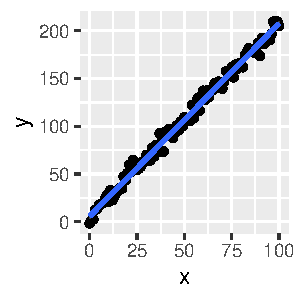
\includegraphics{figs/plot-1} 

}

\caption[R plot]{R plot}\label{fig:plot}
\end{figure}
\end{CodeChunk}

\hypertarget{tables}{%
\subsection{Tables}\label{tables}}

Number tables consecutively; place the table number and title (in 10
point) above the table with one line space above the caption and one
line space below it, as in Table 1. You may float tables to the top or
bottom of a column, set wide tables across both columns.

You can use the xtable function in the xtable package.

\begin{table}[H]
\centering
\begin{tabular}{rrrrr}
  \hline
 & Estimate & Std. Error & t value & Pr($>$$|$t$|$) \\ 
  \hline
(Intercept) & 0.02 & 0.10 & 0.2 & 0.86 \\ 
  x & 2.04 & 0.11 & 19.1 & 0.00 \\ 
   \hline
\end{tabular}
\caption{This table prints across one column.} 
\end{table}

\hypertarget{acknowledgements}{%
\section{Acknowledgements}\label{acknowledgements}}

Place acknowledgments (including funding information) in a section at
the end of the paper.

\hypertarget{references}{%
\section{References}\label{references}}

\setlength{\parindent}{-0.1in} 
\setlength{\leftskip}{0.125in}

\noindent

\hypertarget{refs}{}
\begin{CSLReferences}{1}{0}
\leavevmode\vadjust pre{\hypertarget{ref-Chiu1972}{}}%
Chiu, L. (1972). A cross-cultural comparison of cognitive styles in
chinese and american children. \emph{International Journal of
Psychology}, \emph{7}(4), 235--242.
http://doi.org/\href{https://doi.org/doi:10.1080/00207597208246604}{doi:10.1080/00207597208246604}

\leavevmode\vadjust pre{\hypertarget{ref-Choi1999}{}}%
Choi, I., Nisbett, R. E., \& Norenzayan, A. (1999). Causal attribution
across cultures: Variation and universality. \emph{International Journal
of Psychology}, \emph{125}(1), 47--63.
http://doi.org/\href{https://doi.org/doi:10.1037/0033-2909.125.1.47}{doi:10.1037/0033-2909.125.1.47}

\leavevmode\vadjust pre{\hypertarget{ref-Chua2005}{}}%
Chua, H. F., Boland, J. E., \& Nisbett, R. E. (2005). Cultural variation
in eye movements during scene perception. \emph{Proceedings of the
National Academy of Sciences}, \emph{102}(35), 12629--12633.
http://doi.org/\href{https://doi.org/10.1073/pnas.0506162102}{10.1073/pnas.0506162102}

\leavevmode\vadjust pre{\hypertarget{ref-COCA}{}}%
Davies, M. (2008-2008-). The corpus of contemporary american english
(COCA). Retrieved from \url{https://www.english-corpora.org/coca/}

\leavevmode\vadjust pre{\hypertarget{ref-Francis2005}{}}%
Francis, W. S. (2005). \emph{Bilingual semantic and conceptual
representation}. Oxford University Press.

\leavevmode\vadjust pre{\hypertarget{ref-VICorpus}{}}%
Goldhahn, D., Eckart, T., \& Quasthoff, U. (2012). Building large
monolingual dictionaries at the leipzig corpora collection: From 100 to
200 languages. Retrieved from
\url{https://wortschatz.uni-leipzig.de/en/download/vietnamese}

\leavevmode\vadjust pre{\hypertarget{ref-Grave2018}{}}%
Grave, E., Bojanowski, P., Gupta, P., Joulin, A., \& Mikolov, T. (2018).
Learning word vectors for 157 languages. In \emph{Proceedings of the
international conference on language resources and evaluation (LREC
2018)}.

\leavevmode\vadjust pre{\hypertarget{ref-Griffiths2007}{}}%
Griffiths, T. L., Steyvers, M., \& Tenenbaum, J. B. (2007). Topics in
semantic representation. \emph{Psychological Review}, \emph{114}(2),
211--244.
http://doi.org/\href{https://doi.org/doi:10.1037/0033-295x.114.2.211}{doi:10.1037/0033-295x.114.2.211}

\leavevmode\vadjust pre{\hypertarget{ref-Hui2002}{}}%
Hui, W. (2002). Modernity and 'asia' in the study of chinese history. In
E. Fuchs \& B. Stuchteyi (Eds.), \emph{Across cultural borders:
Historiography in global perspective}. Rowman \& Littlefield.

\leavevmode\vadjust pre{\hypertarget{ref-Jatnika2019}{}}%
Jatnika, D., Bijaksana, M. A., \& Suryani, A. A. (2019). Word2Vec model
analysis for semantic similarities in english words. \emph{Procedia
Computer Science}, \emph{157}, 160--167.
http://doi.org/\url{https://doi.org/10.1016/j.procs.2019.08.153}

\leavevmode\vadjust pre{\hypertarget{ref-Ji2000}{}}%
Ji, L., Peng, K., \& Nisbett, R. E. (2000). Culture, control, and
perception of relationships in the environment. \emph{Journal of
Personality and Social Psychology}, \emph{78}(5), 943--955.
http://doi.org/\href{https://doi.org/doi:10.1037/0022-3514.78.5.943}{doi:10.1037/0022-3514.78.5.943}

\leavevmode\vadjust pre{\hypertarget{ref-Ji2004}{}}%
Ji, L., Zhang, Z., \& Nisbett, R. E. (2004). Is it culture or is it
language? Examination of language effects in cross-cultural research on
categorization. \emph{Journal of Personality and Social Psychology},
\emph{87}(1), 57--65.
http://doi.org/\href{https://doi.org/doi:10.1037/0022-3514.87.1.57}{doi:10.1037/0022-3514.87.1.57}

\leavevmode\vadjust pre{\hypertarget{ref-Liu2019}{}}%
Liu, N., Feng, C., Wu, S., Chan, A., \& Fulton, J. (2019). Automate RFP
response generation process using FastText word embeddings and soft
cosine measure. In \emph{Proceedings of the 2019 international
conference on artificial intelligence and computer science} (pp.
12--17).
http://doi.org/\href{https://doi.org/10.1145/3349341.3349362}{10.1145/3349341.3349362}

\leavevmode\vadjust pre{\hypertarget{ref-Markman1984}{}}%
Markman, E. M., \& Hutchinson, J. E. (1984). Children's sensitivity to
constraints on word meaning: Taxonomic versus thematic relations.
\emph{Cognitive Psychology}, \emph{16}(1), 1--27.
http://doi.org/\href{https://doi.org/doi:10.1016/0010-0285(84)90002-1}{doi:10.1016/0010-0285(84)90002-1}

\leavevmode\vadjust pre{\hypertarget{ref-Masuda2001}{}}%
Masuda, T., \& Nisbett, R. E. (2001). Attending holistically versus
analytically: Comparing the context sensitivity of japanese and
americans. \emph{Journal of Personality and Social Psychology},
\emph{81}(5), 922--934.
http://doi.org/\href{https://doi.org/doi:10.1037/0022-3514.81.5.922}{doi:10.1037/0022-3514.81.5.922}

\leavevmode\vadjust pre{\hypertarget{ref-Mikolov2018}{}}%
Mikolov, T., Grave, E., Bojanowski, P., Puhrsch, C., \& Joulin, A.
(2018). Advances in pre-training distributed word representations. In
\emph{Proceedings of the international conference on language resources
and evaluation (LREC 2018)}.

\leavevmode\vadjust pre{\hypertarget{ref-Nisbett2003}{}}%
Nisbett, R. E. (2003). \emph{The geography of thought: How asians and
westerners think differently \ldots{} and why}. New York: Free Press.

\leavevmode\vadjust pre{\hypertarget{ref-Norenzayan2002}{}}%
Norenzayan, A., Smith, E. E., Kim, B. J., \& Nisbett, R. E. (2002).
Cultural preferences for formal versus intuitive reasoning.
\emph{Cognitive Science}, \emph{26}(5), 653--684.
http://doi.org/\href{https://doi.org/doi:10.1207/s15516709cog2605_4}{doi:10.1207/s15516709cog2605\_4}

\leavevmode\vadjust pre{\hypertarget{ref-Rohde2006}{}}%
Rohde, D. L., Gonnerman, L. M., \& Plaut, D. C. (2006). An improved
model of semantic similarity based on lexical co‐occurrence.
\emph{Communications of the ACM}, \emph{8}, 627--633.

\leavevmode\vadjust pre{\hypertarget{ref-Thompson2020}{}}%
Thompson, R., B., \& Lupyan, G. (2020). Cultural influences on word
meanings revealed through large-scale semantic alignment. \emph{Nature
Human Behaviour Volume}, \emph{4}, 1029--1038.
http://doi.org/\url{https://doi.org/10.1038/s41562-020-0924-8}

\leavevmode\vadjust pre{\hypertarget{ref-2020SciPy}{}}%
Virtanen, P., Gommers, R., Oliphant, T. E., Haberland, M., Reddy, T.,
Cournapeau, D., \ldots{} SciPy 1.0 Contributors. (2020). {{SciPy} 1.0:
Fundamental Algorithms for Scientific Computing in Python}. \emph{Nature
Methods}, \emph{17}, 261--272.
http://doi.org/\href{https://doi.org/10.1038/s41592-019-0686-2}{10.1038/s41592-019-0686-2}

\end{CSLReferences}

\bibliographystyle{apacite}


\end{document}
